\documentclass[a4paper,11pt]{article}
\usepackage[left=2.5cm, right=2.5cm, top=1.5cm, bottom=1.5cm]{geometry}
\usepackage{graphicx}
\usepackage{amssymb}
\usepackage{amsmath}
\usepackage{xcolor}
\usepackage{hyperref}
\usepackage{pythonhighlight}

\hypersetup{ %color attributes of citation, link, etc.
colorlinks=true,
linkcolor=blue,
filecolor=gray,
urlcolor=blue,
citecolor=blue,
}

\setlength{\parindent}{0pt}

% \usepackage[active,tightpage]{preview}
% \renewcommand{\PreviewBorder}{1in}
% \newcommand{\Newpage}{\end{preview}\begin{preview}}

\newcommand{\matlab}{\textsc{Matlab}} %very important and totally necessary addition
\newcommand{\parallelsum}{\mathbin{\!/\mkern-5mu/\!}}

\newcommand\Item[1][]{%
  \ifx\relax#1\relax  \item \else \item[#1] \fi
  \abovedisplayskip=0pt\abovedisplayshortskip=0pt~\vspace*{-\baselineskip}}

%'codify' text for snippets
\usepackage{xcolor}
\definecolor{codegray}{gray}{1}
\newcommand{\code}[1]{\colorbox{codegray}{\texttt{#1}}}
           
\begin{document}
\title{\LARGE{\textbf{Monophonic Mechatronic Chordophone}}}
\author{Daniel Eisen : 300447549\\\textbf{Group Members:} Niels Clayton \& Nickolai Wolfe}
\date{}
\maketitle
\hrule

\section{Introduction}
Core to the design of mechatronic chordophones is the string excitation and damping "loop". This pattern is necessary for the (re)production of music by enabling control over how long a note is sustained by the excited string. 

This report outlines the decisions and motivations in the design/improvement of a pair of picker and damper mechanisms based on identified gaps from systems in literature, first hand experience of a similar systems \cite{mechbass}, and from a set of specifications.

\section{Design Motivations}

The project as a whole was first and foremost aimed at delivering a chordophone that fulfils the following specifications:

\begin{itemize}
  \item 120 pick/damps per minute
  \item Damp string vibrations in 0.25 seconds
  \item Have at least 3 levels of controllable volume 
\end{itemize}

From reviewed literature and experience various areas of the above mechanisms were identified as avenues

\subsection{Potential Picker/Pick Wheel Improvements}
Regarding the performance of this mechanism, this project splits it into two separate sub-mechanisms: The pick-wheel itself and the volume-control.

For this project we decided upon a stepper motor driven pick-wheel due to its simplicity in driving, tested performance \cite{mechbass,singer,Kapur}, and can achieve a high picking speed. 
In literature, the standard approach to the pick-wheel is to flatly fasten a series of picks to some inline mounting drum. Prime examples of this being the mech-bass and LEMUR \cite{mechbass,singer}. From these systems and an in-person demonstration of the mech-bass this project targeted two issues.

This classic approach does however have its own issues and unwanted effectors on the produced sound of the chordophone. 
Around the wheel the picks can be easily mounted miss-aligned, ie slightly offset or rotated, and this can result in a galloping sound with successive pick events. The solid mounting of usually acyclic on PLA additionally cause an audible backlash sound as the pick springs back against its mounting.

On the volume control side, most system in the literature either forgo it entirely or (e.g the MechBass and Strum Bot) have direct servo linkage that puts stain and pressure directly on the shaft in its holding position.

\subsection{Potential Damping Improvements}

In regard to damping mechanisms, our review(s) found that a majority were variations on single contact dampers. This was either achieved with a striking solenoid, \cite{vibe_harp} etc, or a rotating servo with soft interface material, \cite{hammer}.

The result of these approaches is the unwanted displacement of the string, cause an undesirable low frequency pop as it moves over the pick-ups. The obvious solution would be a symmetric actuators, which has been somewhat explored, but requires some design to account for example alignment and impact.

\section{Improved System Designs}

To meets the above goals and specifications this project designed three main mechanisms; Resized Pick-wheel, Rack n' Pinion Volume control which constitute the picker and Duel Leaf Spring Solenoid pair which makes up the damper.

\subsection{Improved Picker Design}

\begin{figure}[h!]
  \begin{center}
    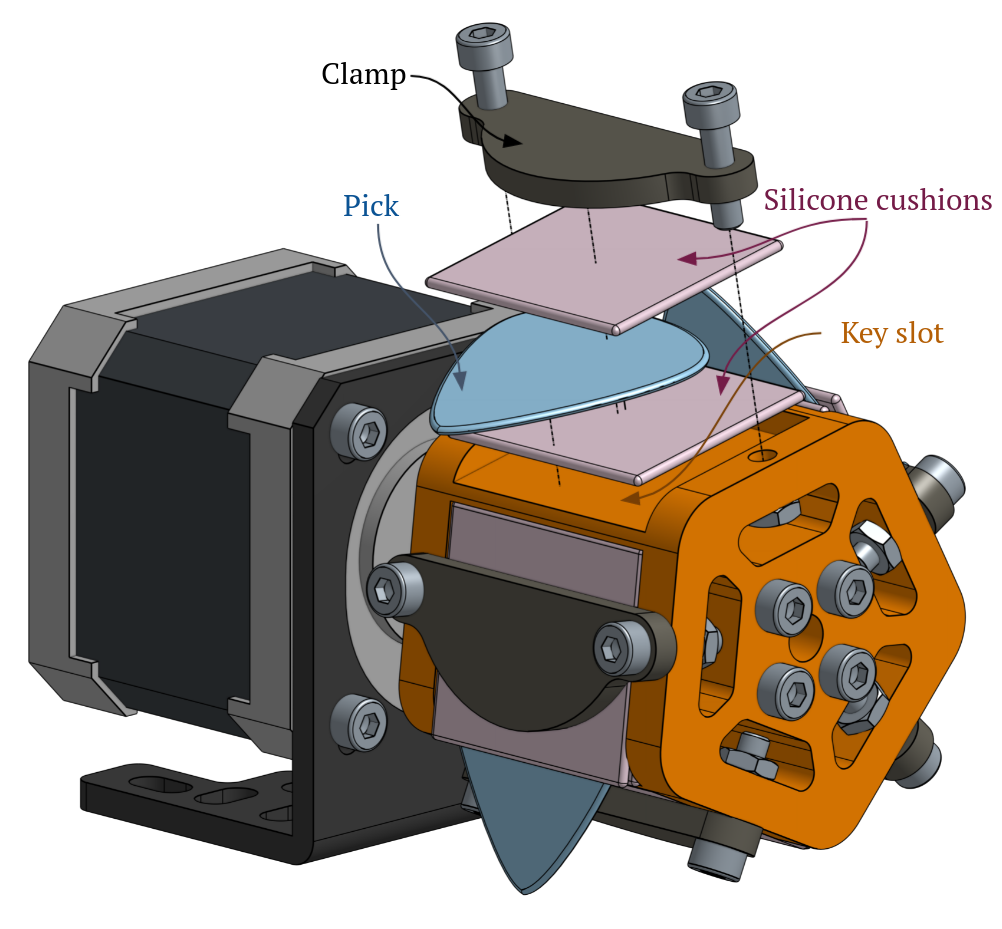
\includegraphics[width=.4\textwidth]{images/picker_explode.png}
    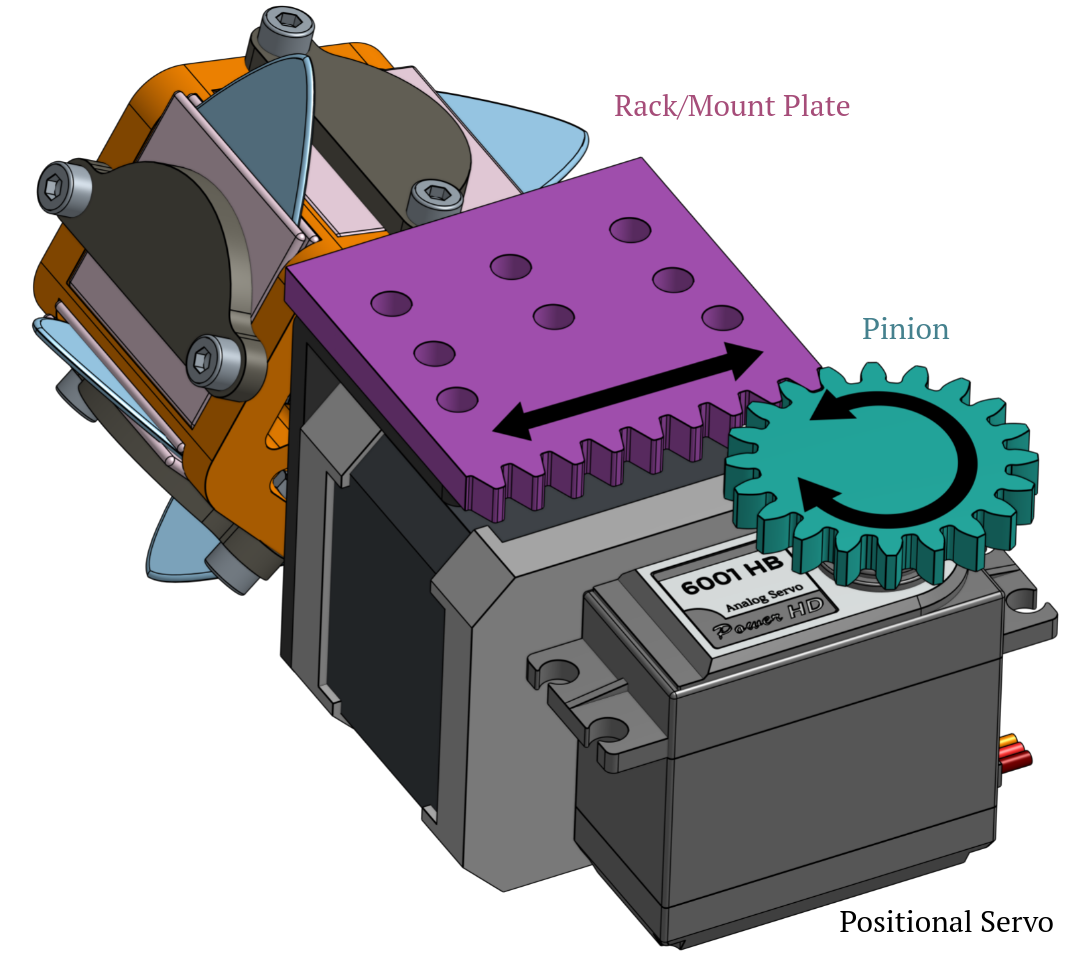
\includegraphics[width=.4\textwidth]{images/volume_explode.png}
    \label{Pick/Vol}
    \caption{Left: Improved Pick-wheel design Right: Rack and Pinion Volume Control Mechanism}
  \end{center}
\end{figure}

A pick-wheel assembly was redesigned from the ground up, with previous designs only as indirect reference, with the aim to account for the aforementioned drawbacks and keeping quality of sound in mind.

\textbf{To address} the misalignment issues and mitigate the associated galloping sound, the wheel is designed to be 3D-printed with keyed slots that match the pick width. This allow the mounting to be tight and prevent them from rotating in place. See left:\ref{Pick/Vol}. The clamp was also extended to spread the pressure to allow to greater positioning and tighter holding force.
To remove the backlash sound the design proposes the pick be clamped between silicone pads. It not only mitigates the harsh slap after a pick but also has the possibility to reintroduce a more nature timbre by loosely imitating a finger-thumb grip.

\textbf{A novel} approach was taken in the design of the volume control. Where our primary goal were to remove static holding pressure from the actuator, allow for high resolution of positioning. The volume is thus modulated by the striking contact area of the pick on string. A positional servo is still used, similar to other systems, due to driving/control simplicity. See Right: \ref{Pick/Vol}, where the pick-wheel is mounted to a baseplate extended into a rack that interfaces with a servo actuated pinion. This removed the servo from holding the resting weight of the assembly and brings it back inline with the stepper for a condensed assembly, see \ref{picker}.

\newpage
\begin{figure}[h!]
  \begin{center}
    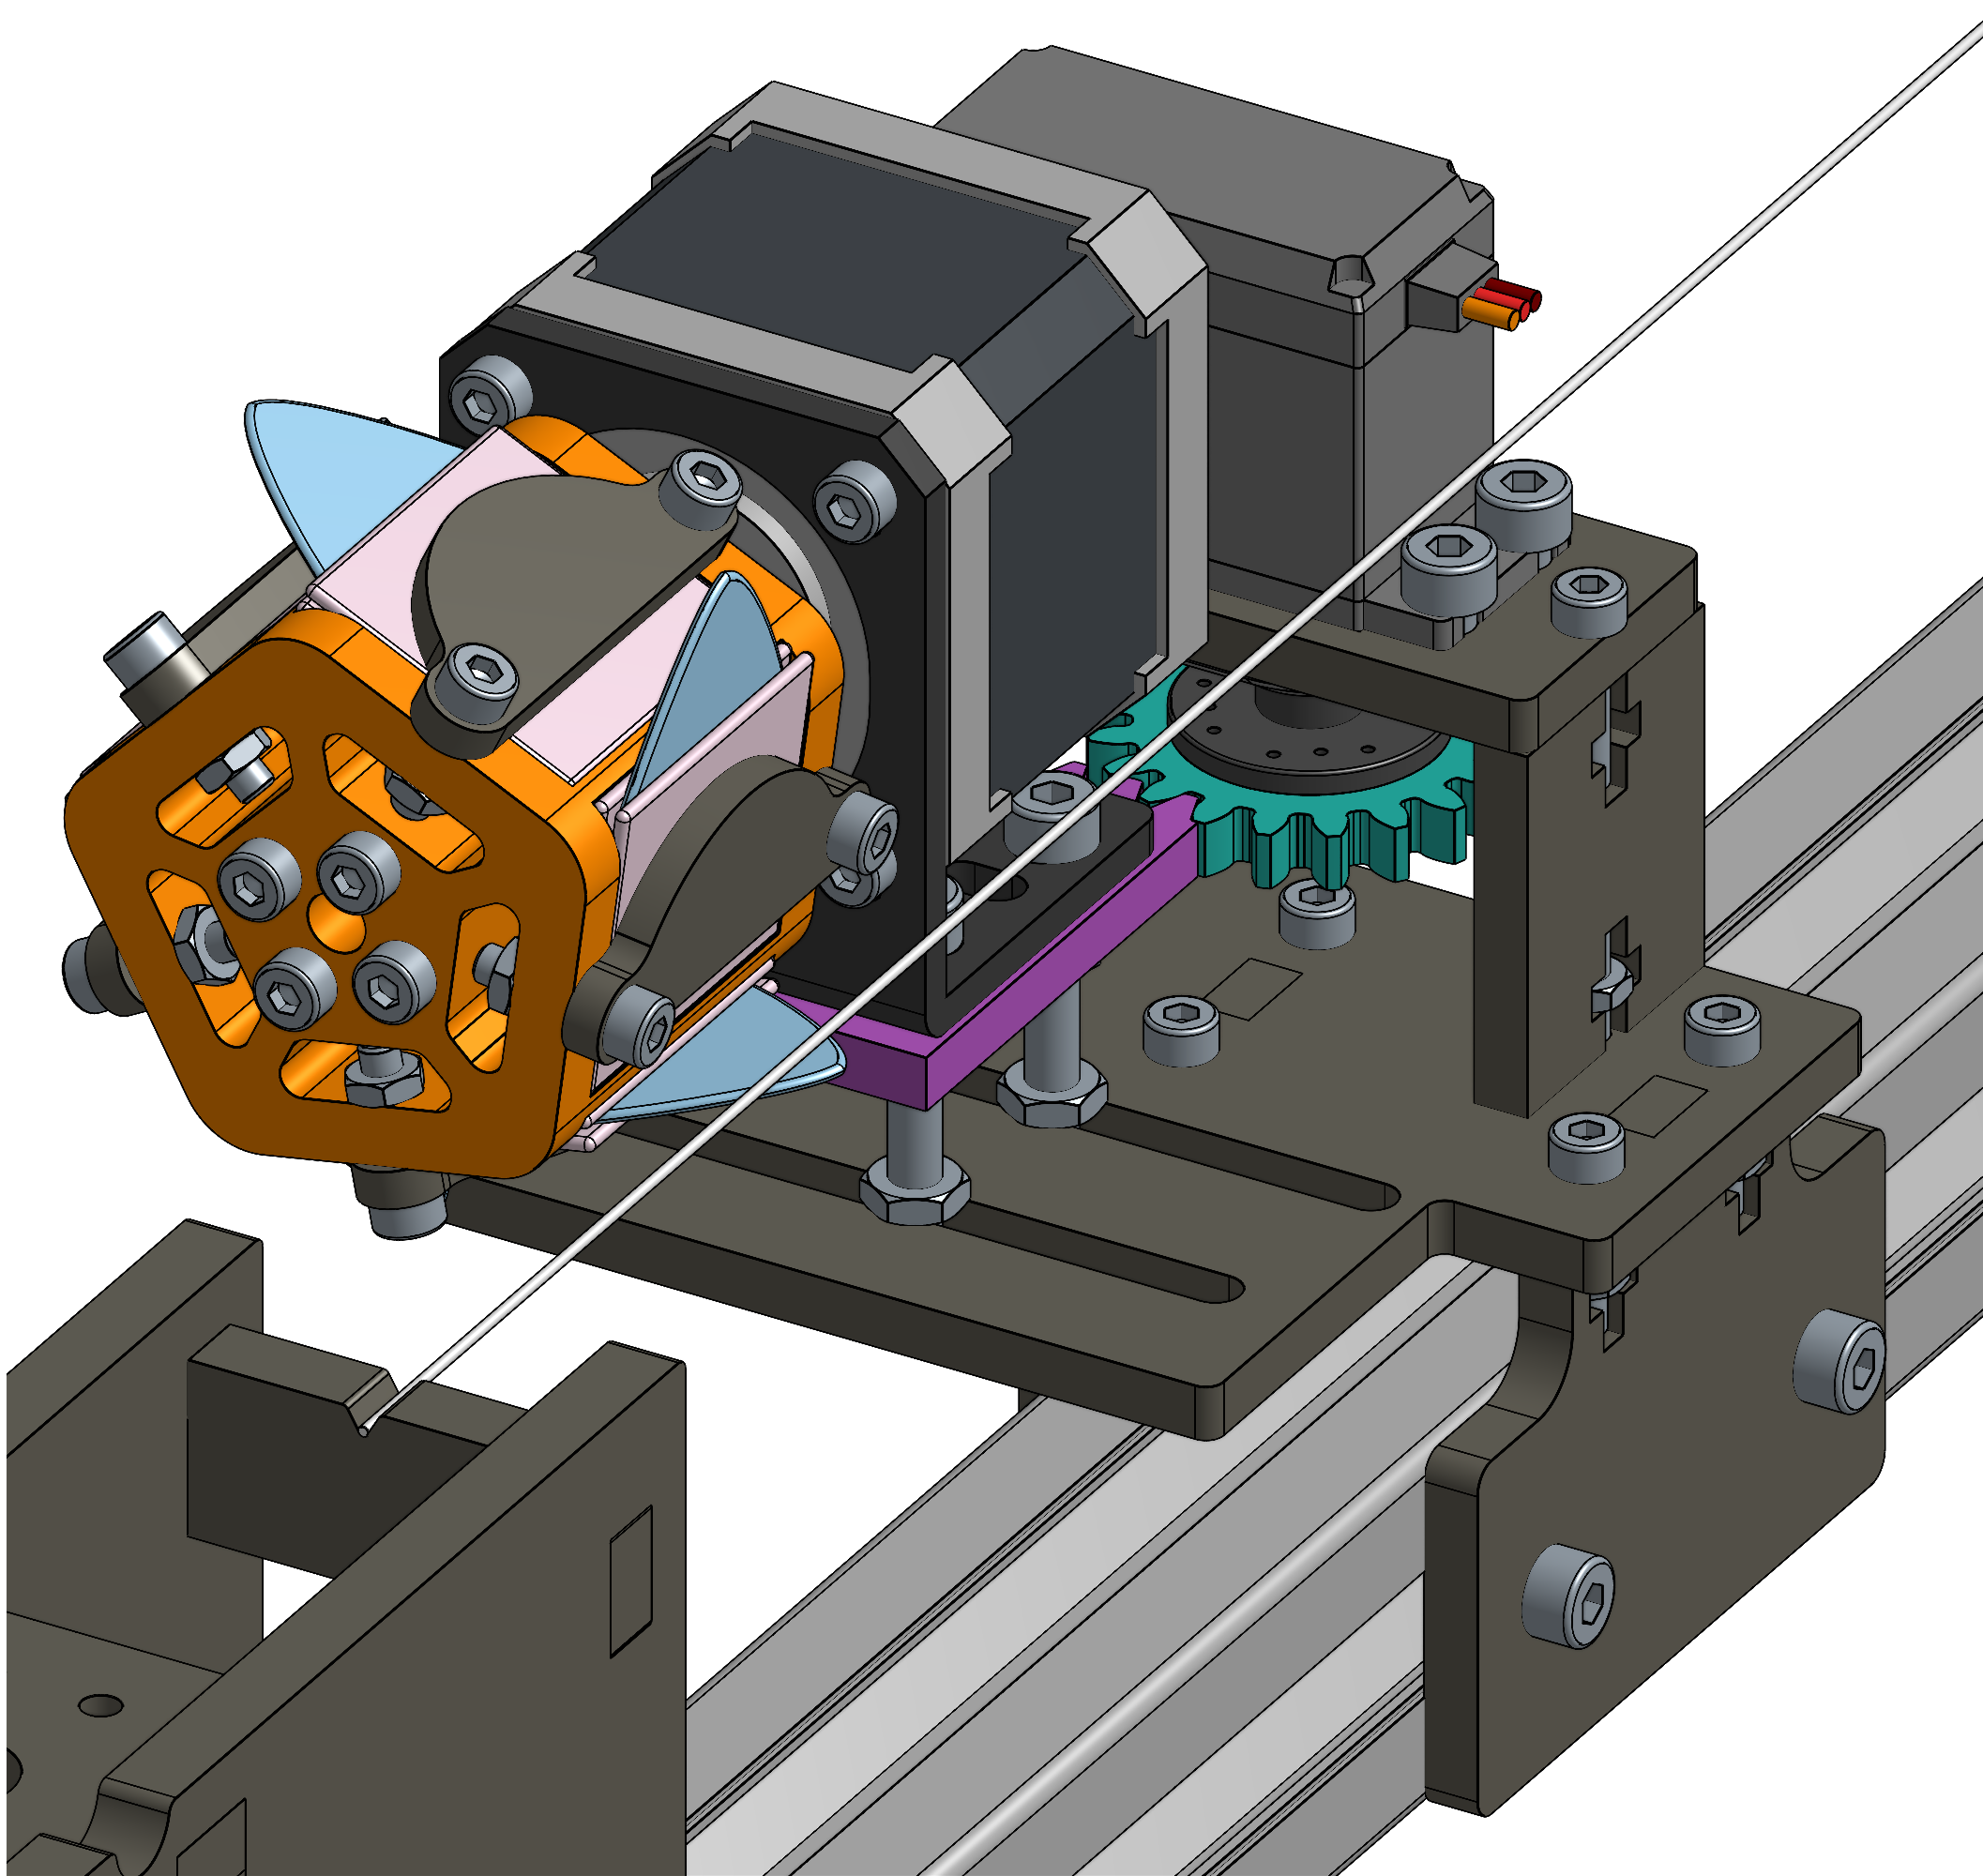
\includegraphics[width=.4\textwidth]{images/picker_assembly.png}
    \caption{Fuller Picker Assembly mounted to extrusion}
    \label{picker}
  \end{center}
\end{figure}

Above \ref{picker}, show the full volume and pick-wheel assembly attached in a sliding mounted base plate. This plate/sliding mechanism is the area most suited for improvement.
Note the that extrusion mounting is sliding for optimum pickup distance (EMI reduction).

\subsection{Improved Damper Design}

\begin{figure}[h!]
  \begin{center}
    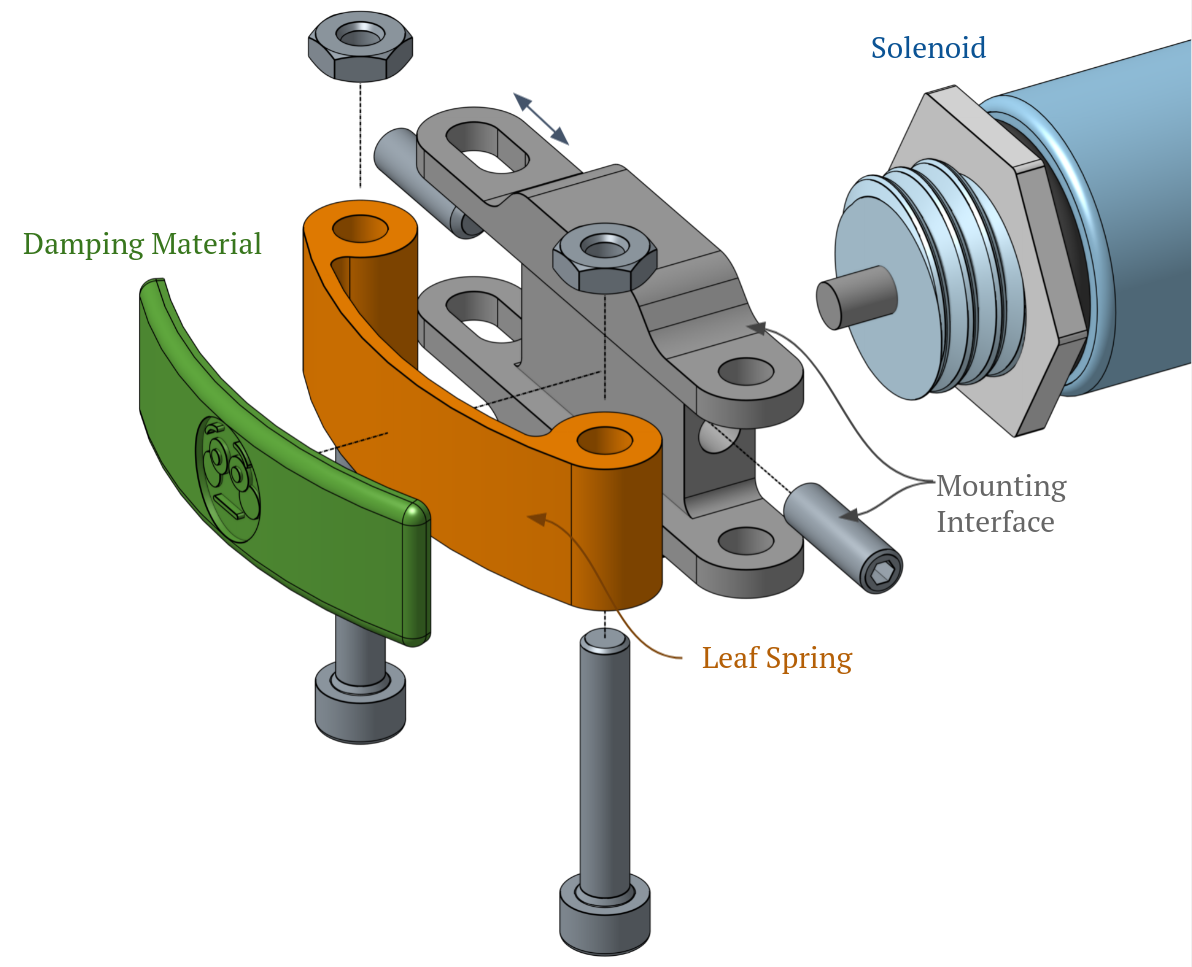
\includegraphics[width=.4\textwidth]{images/damper_explode.png}
    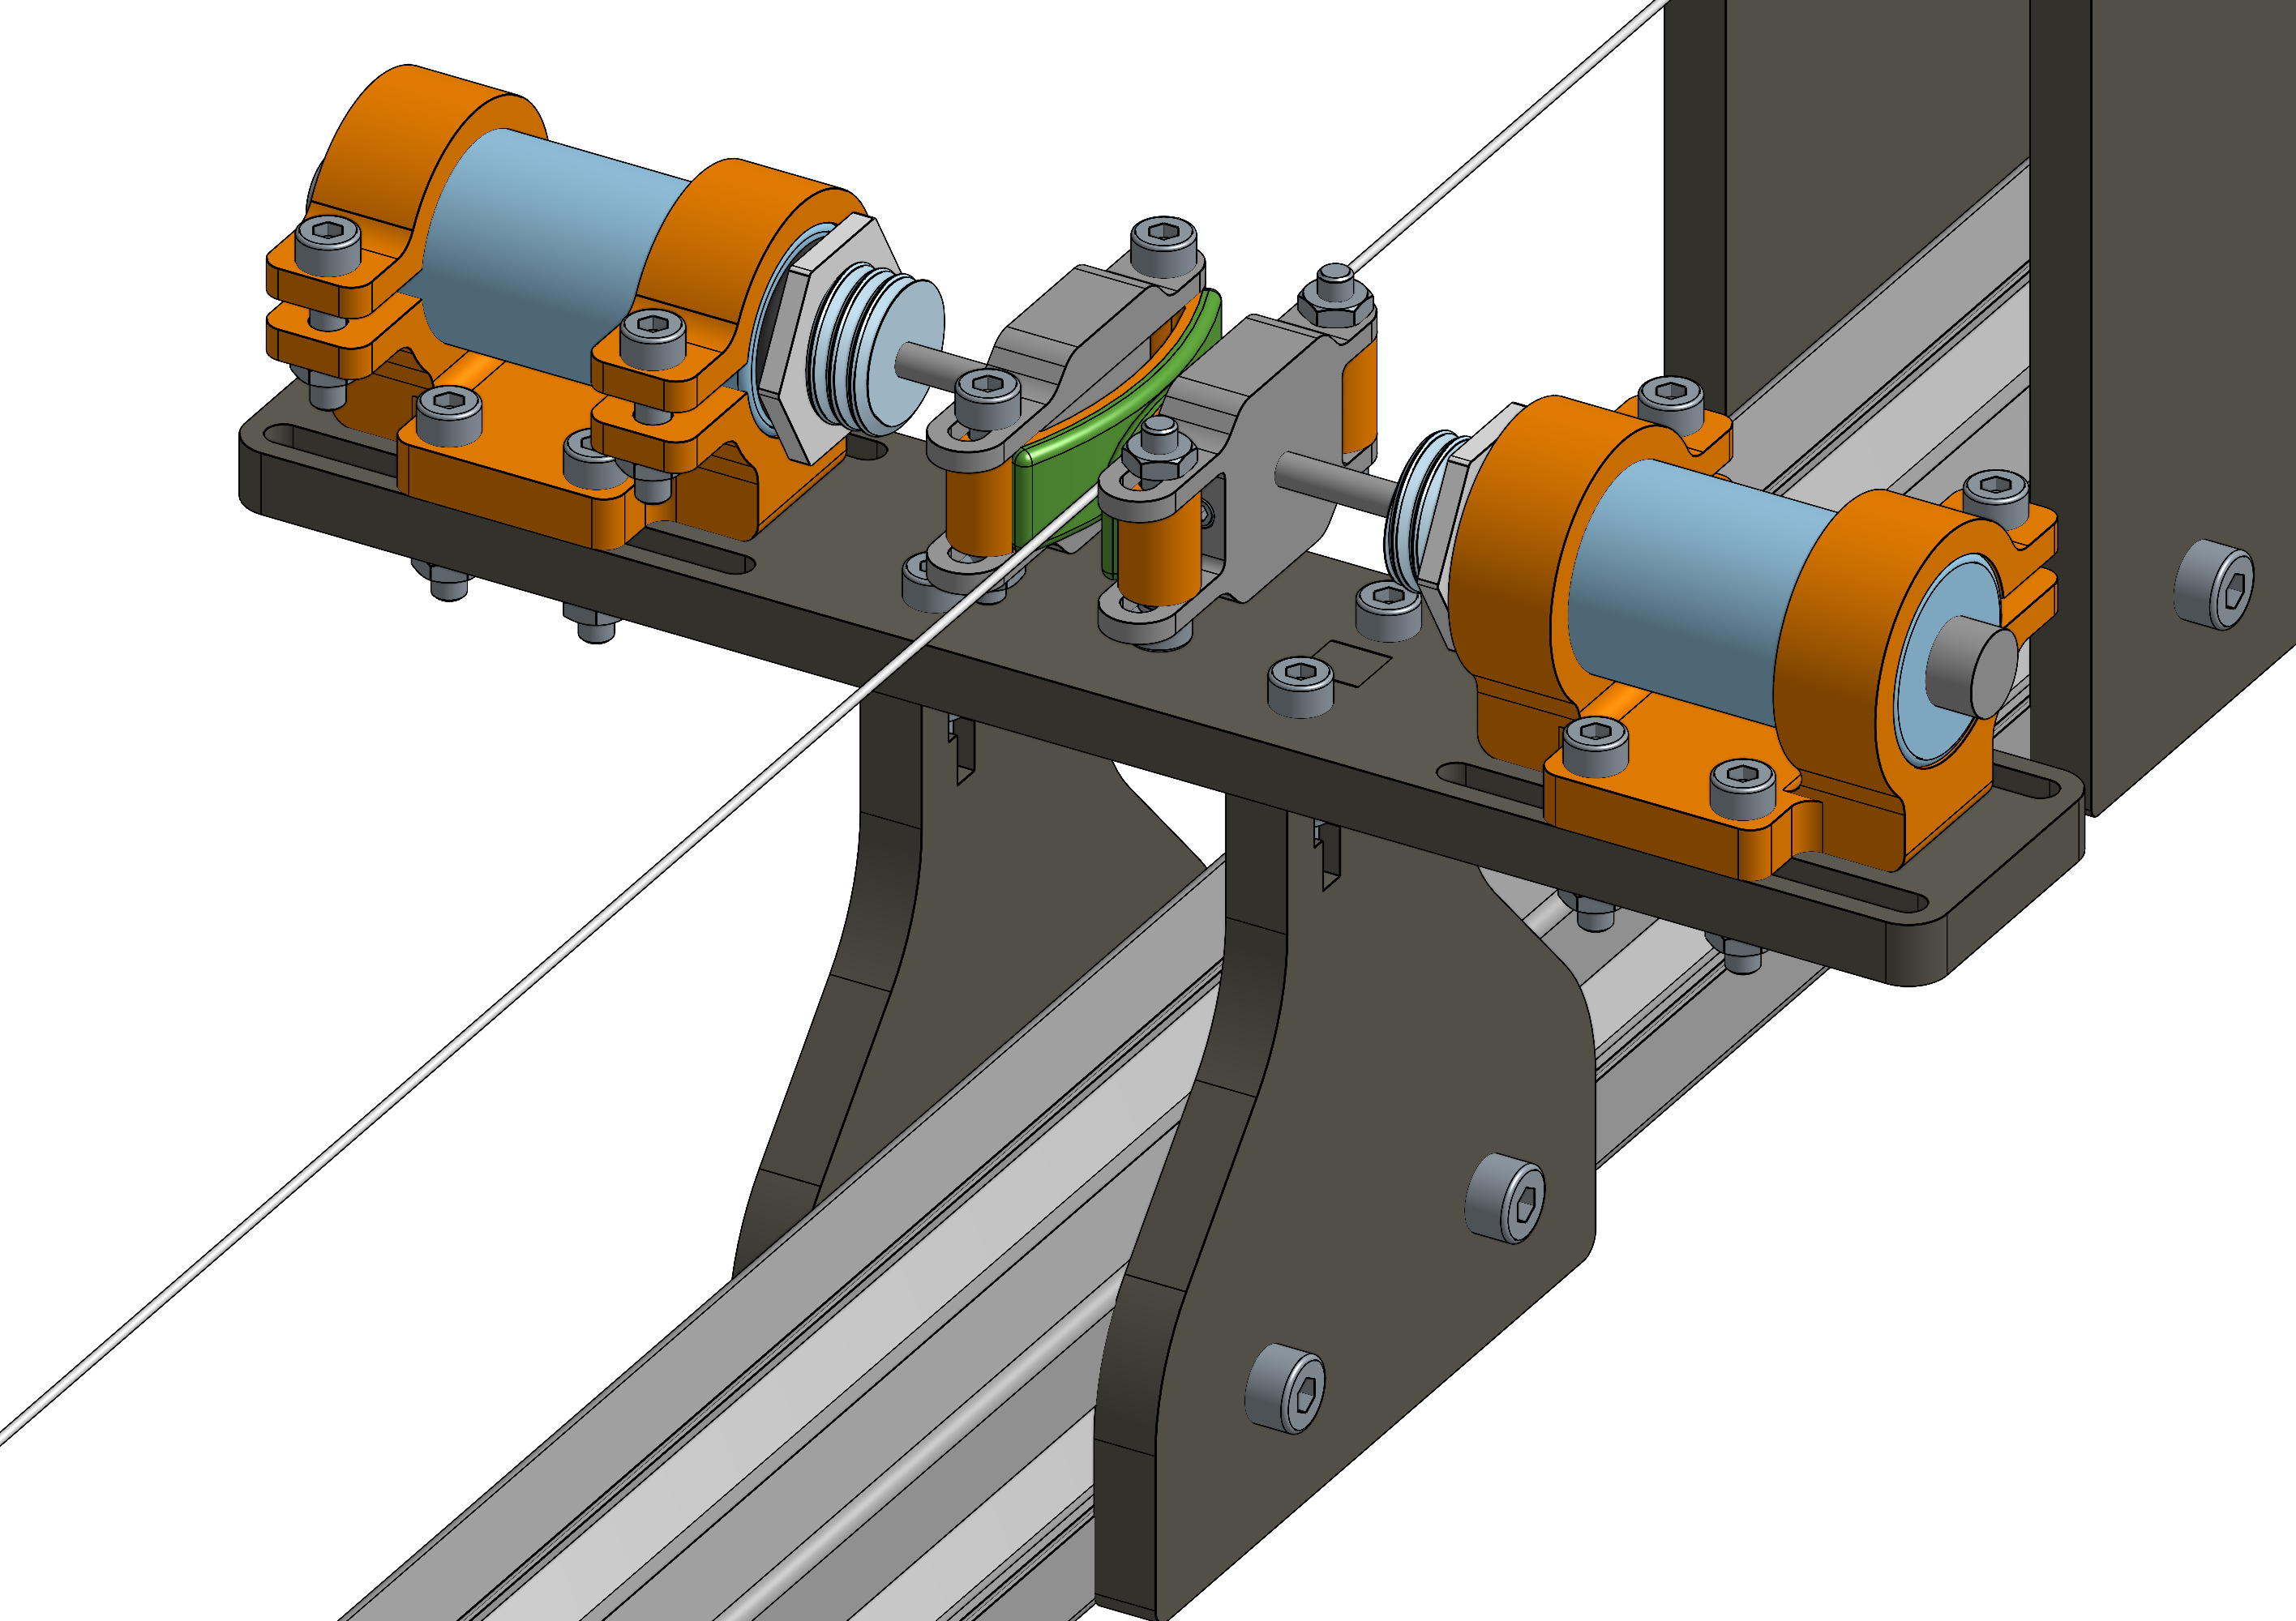
\includegraphics[width=.4\textwidth]{images/damper_assembly.png}
    \label{damp}
  \end{center}
\end{figure}

The major design goal of this system was to mitigate the sting striking displacement as well as compensate for the classic problems associated with our decided approach of pinching solenoids.

Pinching solenoid pairs eliminates the displacement issue, but classically requires matches solenoids, perfect alignment and still can cause a impact pop.
To tackle this leaf spring inspired damper attachments were designed to spread out the force, soften the impact and allow for greater play and tolerance between the actuators. The figure \ref{damp} shows what it uses to achieve this. A soft interface material that can be experimented with to soften the impact sound and absorb some energy, but the meat is taken care of by an leaf spring piece. It is responsible for absorbing the most impact force and smoothing the damping action of the solenoids. It also allows for misalignment as the extension/spread widens the area of contact and eliminated a single node from being damped.

This is slot mounted to a base plate via c-clamps. This allows a strong hold while enabling contact pressure to be adjusted.

\newpage
\subsection{Overall System}

\begin{figure}[h!]
  \begin{center}
    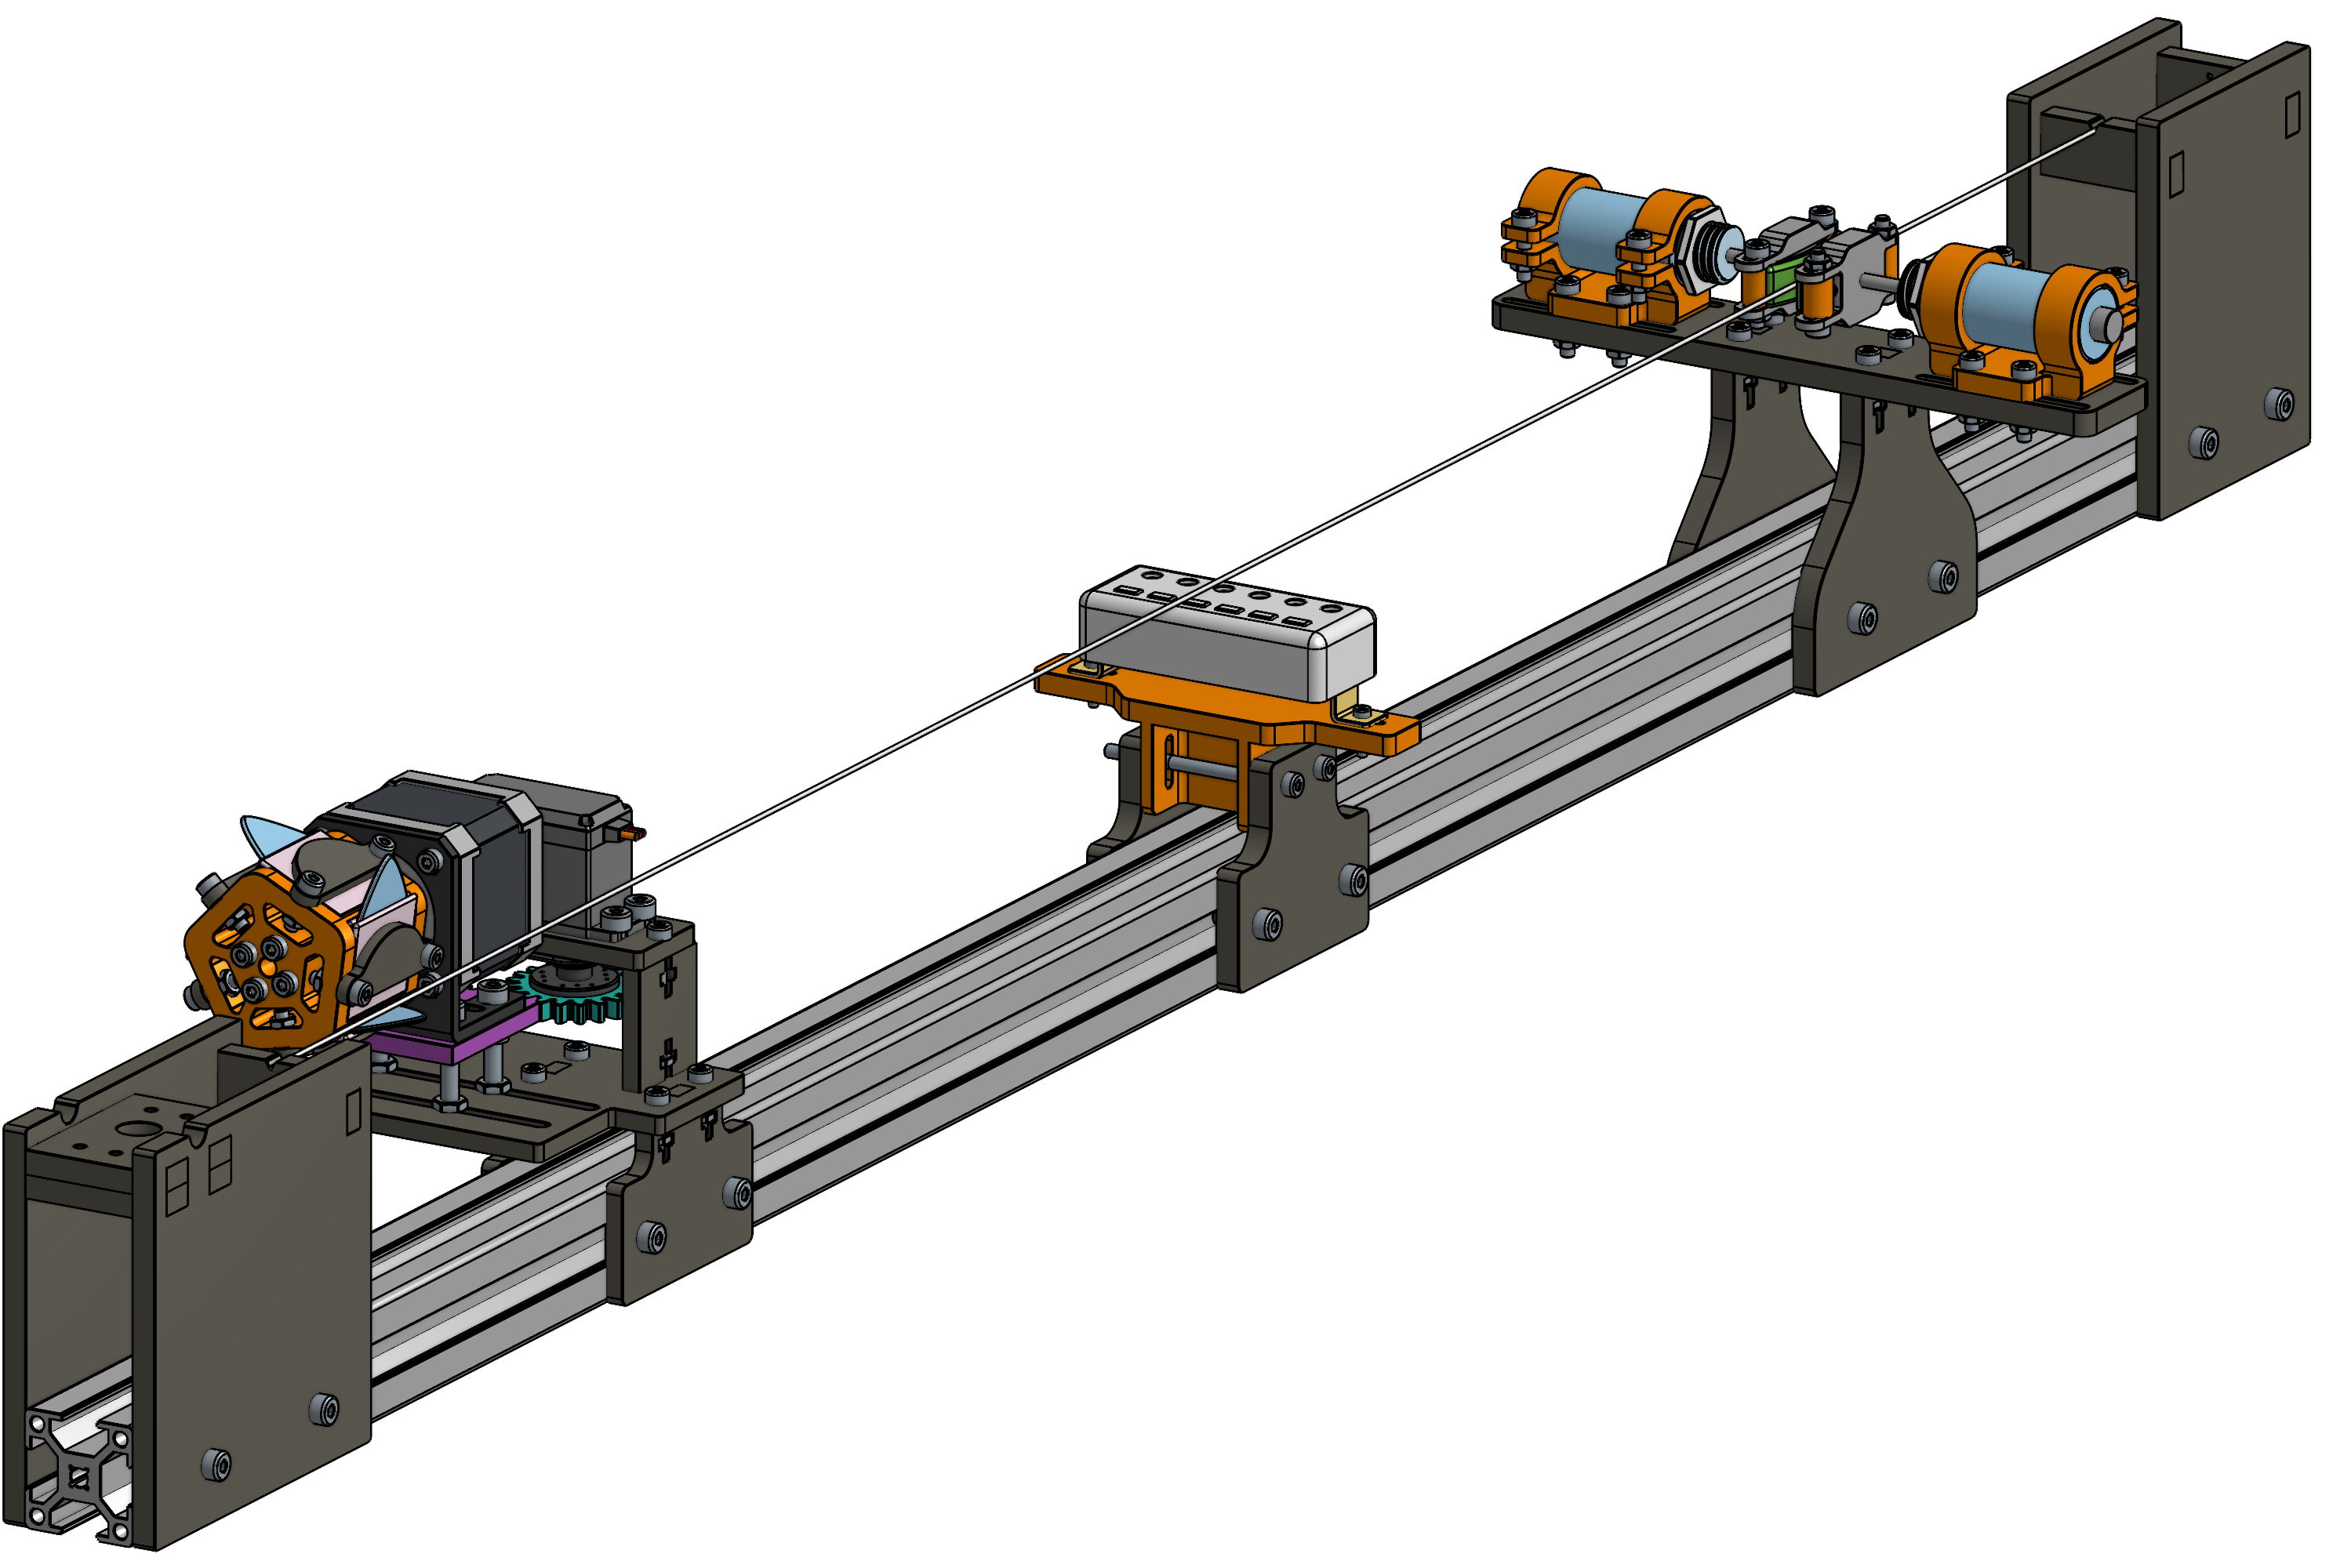
\includegraphics[width=.8\textwidth]{images/picker_damper_full.png}
    \label{Overall}
    \caption{Fully Mounted Chordophone}
  \end{center}
\end{figure}

The figure \ref{Overall} show the fully mounted system, with matching pick-up mount. The mounting allows for each of the modules to have unfixed location that can be tuned to reduced EMI at the pickup.

\subsection{Software API}

\begin{figure} [h!]
  \begin{center}
    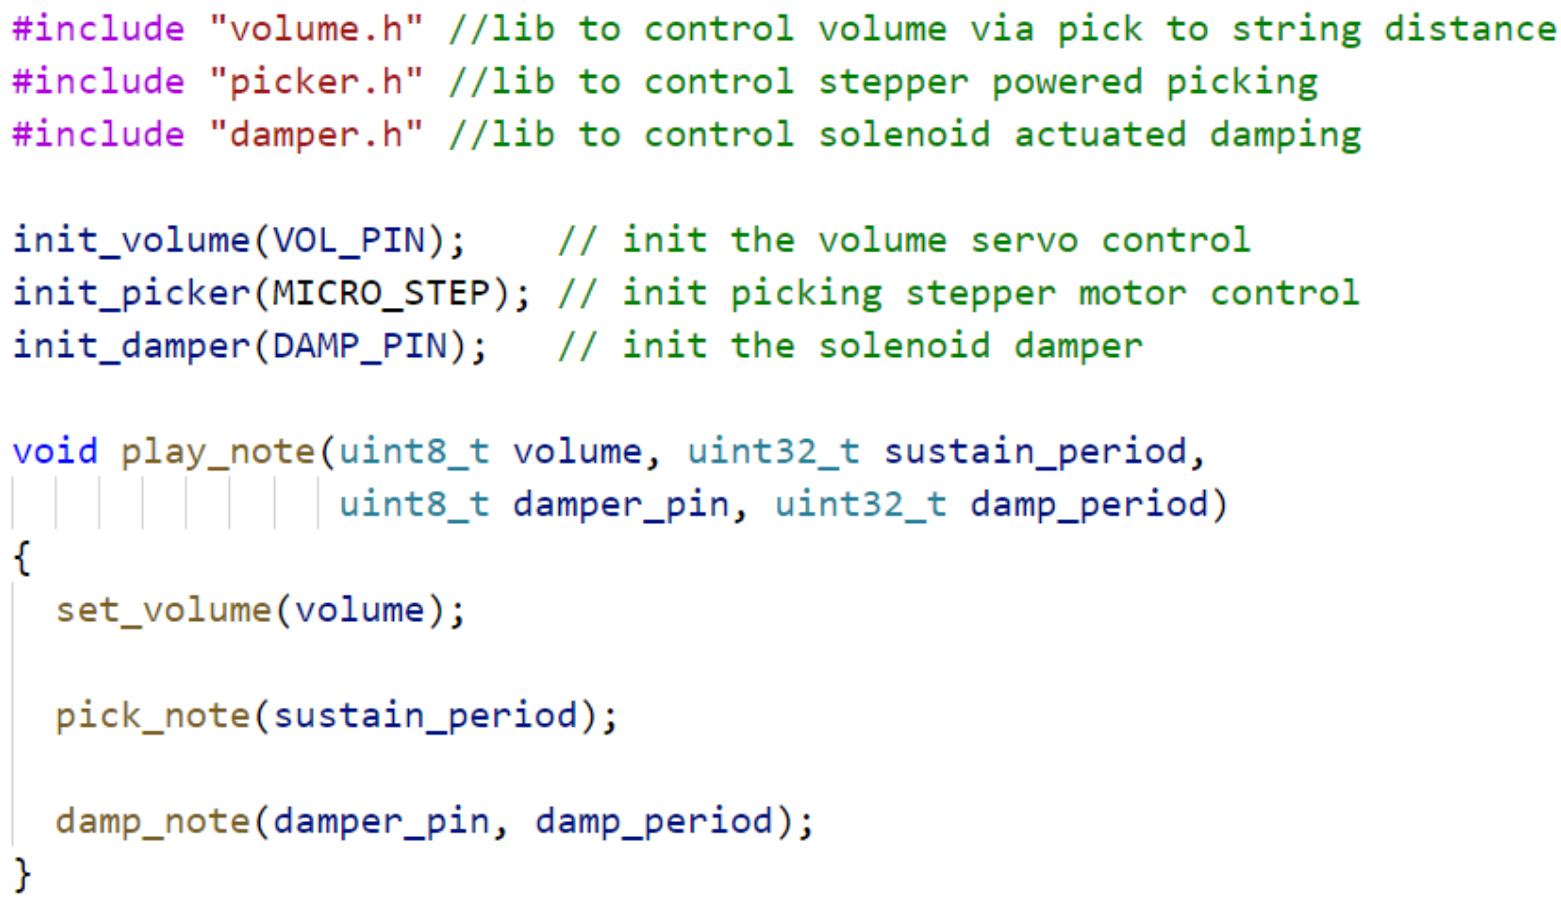
\includegraphics[width=.6\textwidth]{images/code.png}
  \end{center}
\end{figure}

An initial version of an  interfacing API was developed. It consists of 3 independent driving library (headers) and provides a \texttt{play\_note} function that allows a user to set volume, note sustain period, and damping period.    

Volume levels are linearly divided segment of the pick-wheel's min and max positions and supports a resolution up to the positional accuracy of the servo.

Picking utilises the \texttt{FlexyStepper} library to convert pick timings to step signal requirements and generate driving signals. The module also allows for micro-stepping divisions to be programmed to tune for EMI again. 

This API in designed to be easily extended into a fuller MIDI driven system. 

\section{Proposed Evaluation Methods}

Due to COVID-19 restrictions that project never could progressed past the design stage so below describes how its could be reasonably characterised and evaluated. 

\subsection{Picker Evaluation}

To confirm the elimination of the backlash in the picking motion, both the pick-up signals and ambient sounds of the new system and an existing pick wheel can be recorded.
These can be analysed in an audio visualiser or simply played back to whether the solution has worked and removed the clicking and how it affected the integrity of the sound.

To evaluate the pick mounting, long term continuous picking should be performed to check for pick movement, misalignment and/or audible galloping.  

\subsection{Damper Evaluation}
The main evaluation of the damping system would be the comparison of the pick-up signals of a single actuator, duel spring-less, and full leaf spring dampers.

Analysing for mitigation of displacement and impact sound.

\section{Conclusion and Future Work}

Other than a robust evaluation and iteration upon the current design, future extensions of this project may involve a more thought out version of the picker sliding mount. The API and software represents the majority of the projects extendibility; MIDI integration, end-user friendly interface program more music generation features etc.

In conclusion this project produced a robust and very build friendly design. 
The stepper driven pick wheel would allow for much higher than he required 120 p/m. The dampers remain untested, so no confirmation can be stated whether it achieves $<0.25s$. The combination of rack and pinion and servo driving volume library allows for much greater than 3 levels of volume change and can be set per note/pick.


\newpage
\bibliography{ref}
\bibliographystyle{IEEEtran}
\end{document}